
\documentclass[xcolor=x11names,compress,10pt,handout]{beamer}

%% Beamer Layout %%%%%%%%%%%%%%%%%%%%%%%%%%%%%%%%%%
\useoutertheme[subsection=false,shadow]{miniframes}
\useinnertheme{default}
\usefonttheme{serif}
%\usepackage{palatino}

\usepackage{listings}
\usepackage{courier}
\lstset{basicstyle=\footnotesize\ttfamily,breaklines=true}
\lstset{
  backgroundcolor=\color{white!90!blue},
  basicstyle=\footnotesize\tt,     % the size of the fonts that are used for the code
  breakatwhitespace=false,         % sets if automatic breaks should only happen at whitespace
  breaklines=true,                 % sets automatic line breaking
  captionpos=b,                    % sets the caption-position to bottom
  extendedchars=true,              % lets you use non-ASCII characters; for 8-bits encodings only, does not work with UTF-8
  frame=single,                    % adds a frame around the code
  keywordstyle=\bf,
  showspaces=false,                % show spaces everywhere adding particular underscores; it overrides 'showstringspaces'
  showstringspaces=false,          % underline spaces within strings only
  showtabs=false,                  % show tabs within strings adding particular underscores
  tabsize=2                        % sets default tabsize to 2 spaces
}

\setbeamercolor*{lower separation line head}{bg=Firebrick4} 
\setbeamercolor*{normal text}{fg=black,bg=white} 
\setbeamercolor*{alerted text}{fg=red} 
\setbeamercolor*{example text}{fg=black} 
\setbeamercolor*{structure}{fg=Firebrick4} 
 
\setbeamercolor*{palette tertiary}{fg=black,bg=black!10} 
\setbeamercolor*{palette quaternary}{fg=black,bg=black!10} 

\renewcommand{\(}{\begin{columns}}
\renewcommand{\)}{\end{columns}}
\newcommand{\<}[1]{\begin{column}{#1}}
\renewcommand{\>}{\end{column}}


\newenvironment<>{block1}[1]{%
  \setbeamercolor{block title}{fg=black,bg=Firebrick4!15!white}%
  \begin{block}#2{#1}}{\end{block}}
  
  
\newenvironment<>{block2}[1]{%
  \setbeamercolor{block title}{fg=white,bg=blue!75!black}%
  \begin{block}#2{#1}}{\end{block}}

\newcommand{\by}{\mathbf{y}}
\newcommand{\bphi}{\boldsymbol{\phi}}

\setbeamercolor{block body}{fg=black,bg=gray!7}

\usepackage[absolute,overlay]{textpos}

% LOGO
\newcommand\FrameText[1]{%
  \begin{textblock*}{0.8\paperwidth}(40pt,.82\textheight)
    \raggedright #1\hspace{.5em}
  \end{textblock*}}
  
%\setbeamerfont{title like}{shape=\scshape}
\setbeamerfont{frametitle}{shape=\bf} 

\begin{document}


%%%%%%%%%%%%%%%%%%%%%%%%%%%%%%%%%%%%%%%%%%%%%%%%%%%%%%
%%%%%%%%%%%%%%%%%%%%%%%%%%%%%%%%%%%%%%%%%%%%%%%%%%%%%%
\begin{frame}
\title[]{\LARGE\bf\textcolor{black}{Statistical inference for ERGMs}}
\subtitle[]{(Chapter 4 \& 5 of the manual)}
  
\author[]{\large\textcolor{Firebrick4}{\bf Alberto Caimo}\\ 
          }

\institute[]
  {\sc\normalsize Dublin Institute of Technology\\
   Ireland}

\date[]
  {}

\titlepage
 
 \FrameText{ \centering
 
\includegraphics[width=.8\textwidth]{ssnar_logo_slides}}

\end{frame}


%%
%\begin{frame}{Outline}
%\tableofcontents
%\end{frame}

%%
% \begin{itemize}
% \item
% \end{itemize}

%
\begin{frame}[fragile]{} 
\begin{center}
{\LARGE \bf Classical inference for ERGMs} 
\end{center}
\end{frame}

%
\begin{frame}[fragile]{Model specification} 
\begin{itemize}
\item ERGM specification = choice of network statistics $s(y)$ to include in the model;
\item The first statistics $s_1(y) =$ number of edges, it's a sort of baseline density effect;
\item The other statistics are selected according to the type of effects we are interested in.
\end{itemize}
\vspace{.5cm}
For example:
\begin{lstlisting}
library(statnet)
load(url("https://acaimo.github.io/lazega.RData"))
y <- network(Y, directed = FALSE)
model.1.0 <- y ~ edges + kstar(2) + triangle
\end{lstlisting}
\end{frame}

%
\begin{frame}[fragile]{Degeneracy} 
\begin{itemize}
\item To estimate an ERGM we can use the {\tt ergm()} function;
\item \textcolor{red}{ATTENTION!} Some ERGM specifications lead to a {\bf degenerate} model which may not be estimated
\end{itemize}
\vspace{.5cm}
For example:
\begin{lstlisting}
model.1.0 <- y ~ edges + kstar(2) + triangle
ergm(model.1.0)
\end{lstlisting}
\end{frame}

%
\begin{frame}[fragile]{Higher-order network statistics} 
\begin{itemize}
\item In order to try to overcome degeneracy issues, a new specification of network statistics based on geometrically weighted functions of extra-triadic network statistics distributions have been proposed by Snijders et al. (2006);
\item This statistics include, for example: \\
- geometrically-weighted degree ({\tt gwdegree}) statistic (replacing the stars) \\
- geometrically-weighted edgewise shared partner ({\tt gwesp}) statistic (replacing triangles) 
\end{itemize}
\end{frame}

%
\begin{frame}[fragile]{ERGMs in action} 

For example:
\begin{lstlisting}
model.1.1 <- y ~ edges + 
                 gwdegree(1, fixed = TRUE) + 
                 gwesp(1, fixed = TRUE)
MLE.1.1 <- ergm(model.1.1)
summary(MLE.1.1)

 ## Monte Carlo MLE Results:
 ##               Estimate Std. Error MCMC % p-value    
 ## edges          -4.1437     0.5667      0  <1e-04 ***
 ## gwdegree        0.7340     0.4580      0   0.109    
 ## gwesp.fixed.1   0.9327     0.1716      0  <1e-04 ***
 ## ---
 ## Signif. codes:  0 '***' 0.001 '**' 0.01 '*' 0.05 '.'
 ## 
 ## AIC: 524.4    BIC: 537.7    (Smaller is better.)
\end{lstlisting}
\end{frame}

%
\begin{frame}[fragile]{ERGMs in action}  

Another example with covariate information:
\begin{lstlisting}
# Add attributes to the network object y:
set.vertex.attribute(y, "Office", X$Office)
set.vertex.attribute(y, "Years", X$Years)

model.2 <- y ~ edges + 
               nodematch("Office") +
               nodecov("Years") +
               gwesp(0.6, fixed = TRUE) +
               gwdegree(0.6, fixed = TRUE)

MLE.2 <- ergm(model.2)
summary(MLE.2)
\end{lstlisting}
\end{frame}

%
\begin{frame}[fragile]{ERGMs in action} 

Another example with covariate information (cont'd):
\begin{lstlisting}
 ## Monte Carlo MLE Results:
 ##                   Estimate Std. Error MCMC % p-value    
 ## edges            -4.309415   0.617740      0  <1e-04 ***
 ## nodematch.Office  0.878821   0.174202      0  <1e-04 ***
 ## nodecov.Years    -0.013317   0.005855      0  0.0233 *  
 ## gwesp.fixed.0.6   1.385871   0.276452      0  <1e-04 ***
 ## gwdegree          0.360304   0.619493      0  0.5610    
 ## ---
 ## Signif. codes:  0 '***' 0.001 '**' 0.01 '*' 0.05 '.'
 ##  
 ## AIC: 500.6    BIC: 522.9    (Smaller is better.) 
\end{lstlisting}
\end{frame}

%
\begin{frame}[fragile]{Output diagnostics} 
\begin{lstlisting}
mcmc.diagnostics(MLE.2)
\end{lstlisting}
 \begin{center}
 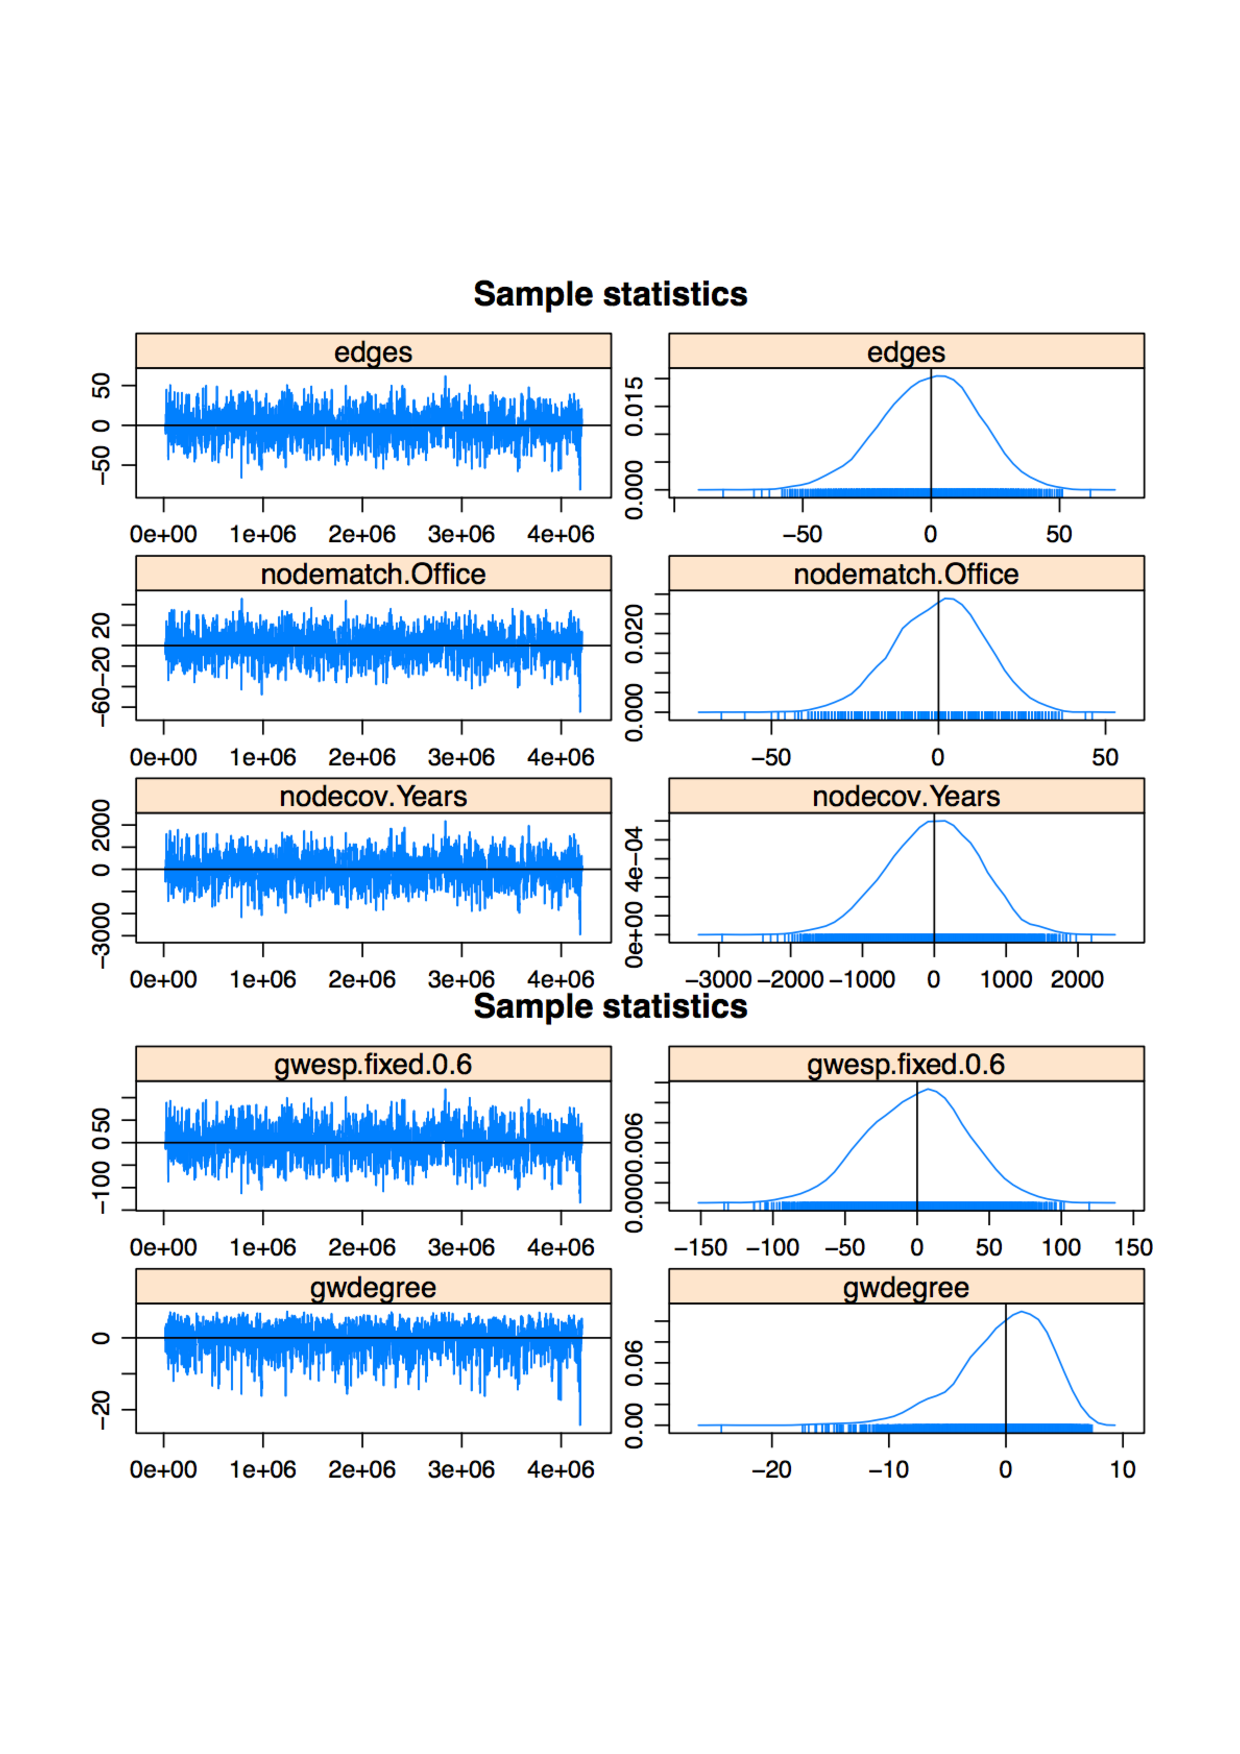
\includegraphics[scale=0.32]{MLE_diagnostics.pdf}
 \end{center}
\end{frame}

% 
\begin{frame}[fragile]{Goodness of fit diagnostics}
\begin{itemize}
\item If the estimated ERGM is a good fit to the observed data, then networks simulated $y_1, \dots, y_m$ should resemble the connectivity structure of the observed data $y$. 
\item To do this, $M$ graphs are simulated from the MLE of the parameter $\hat{\theta}$ and compared to the observed graph in terms of high-level network statistics $g(y)$ which are not modelled explicitly.
\item We expect that:
$$
E(g(\tilde{y})) = \frac{1}{M} \sum_{i = 1}^{M} g(\tilde{y_i}) \approx g(y);
$$
\end{itemize}
\end{frame}


% 
\begin{frame}[fragile]{Goodness of fit diagnostics}
\begin{lstlisting}
par(mfrow = c(2, 2))
plot(model.2.gof, main = '')
\end{lstlisting}
 \begin{center}
 \includegraphics[scale=0.4]{GOF.pdf}
 \end{center}
\end{frame}

\end{document}














